\chapter[Introduction]{Introduction}{Introduction}\label{CH1:Intro}

\section{Background}
Lean combustion is utilized across various sectors of combustion technologies, including boilers, internal combustion engines, furnaces, and gas turbines. The broad application range aims to capitalize under fuel lean conditions on the benefits of operating combustion processes, which offer both high efficiency and low emissions. By maintaining low flame temperatures, pollutant emissions are effectively reduced, particularly in terms of thermal nitric oxide formation. Furthermore, when lean conditions are achieved with excess air during hydrocarbon combustion, complete fuel burnout is typically achieved, resulting in decreased emissions of hydrocarbons and carbon monoxide. However, implementing these enhancements and meeting the practical requirements of combustion systems is challenging due to factors such as slow reaction rates, the possibility of extinction, sensitivity to mixing, instability, and mild heat release.

Emerging technology of Colourless Distributed Combustion (CDC) \cite{VAThesis2011,VA2011} has the potential to meet the stringent demands for reduced pollution and improved reliability in upcoming gas turbine technologies. Low emission of nitrogen oxides (NOx) is a crucial characteristic of gas turbine engines. Concentrated release of aircraft emissions in specific regions and the lower stratosphere intensifies the impact of the aviation industry's relatively small contribution to overall emissions. Land-based gas turbine engines contribute significantly to NOx and CO emissions, alongside aviation-related gas turbine engines. High demand for power generation engines can be attributed to their lower capital investment costs, superior thermodynamic efficiencies, and current affordability of natural gas. Increasing stringency of environmental regulations concerning NOx emissions for gas turbines and other power generation technologies is a consequential factor that accompanies the growth of gas turbine engines. Implementation of regulations have led to a drive for continuous and extensive research on novel gas turbine combustor technologies, which can effectively mitigate NOx emissions. Potential of colourless distributed combustor to meet power requirements similar to conventional combustors, while also addressing relevant environmental regulations, is a promising development.

In the present study, reverse flow configuration of CDC combustor have been discussed. In this configuration, inlet and outlet are on same side of the combustor. Reverse flow nature of the geometry allows the product gases to recirculate within the combustion chamber and mix with the incoming oxidizer stream and hence diluting it. This drives the combustion towards colorless regime.

\section{Motivation}
Concerns about the effects of pollutants on the environment and health have led to a heightened focus on pollutant emissions. Over the past decades, there have been significant changes in both regulations and technologies aimed at controlling emissions from gas turbines. Additionally, stationary gas turbines have gained prominence in the gas and oil industry, expanding their applications in combined cycle plants and utility power generation. As a result, there is more demand on combustion engineers to reduce pollutant emissions\cite{Lefebvre2009}.

NOx is a concerning pollutant among other pollutants due to its harmful impact on health and contribution to ozone layer depletion. With the growing demand, there is an urgent need to minimize gas turbine engines emissions. Several factors, particularly NOx, have a crucial role in the development of pollutants. Formation of nitrogen oxides (NOx) is primarily influenced by the flame temperature and the duration of combustion products in the chamber. Zeldovich mechanism\cite{LTY2013}, additionally referred to as the thermal NOx mechanism, is one of the various mechanisms for NOx generation and is of utmost significance\cite{LAH2010}. Similar to the NOx produced in just a few milliseconds as the temperature near 2100 K\cite{10.1115/1.4043437}, thermal NOx is produced at roughly 1800 K over a period of time.

Design and development of a novel combustor which can change the dynamics of combustion process to suppress NOx emission will be explored in next chapter.

\section{Gas Turbine Combustor Design Parameters}
There are wide range of basic requirements that a gas turbine needs to satisfy. The geometry of the combustor is determined by certain key factors. Figure \ref{fig:gasTurbineEngine} illustrate a conventional gas turbine combustor highlighting the geometrical aspects of widely used combustion chamber. There could be multiple variations on this fundamental pattern, however, in general, combustion chamber have diffuser, air casing, fuel injector and liner as basic components.
\begin{figure}[ht]
	\centering
	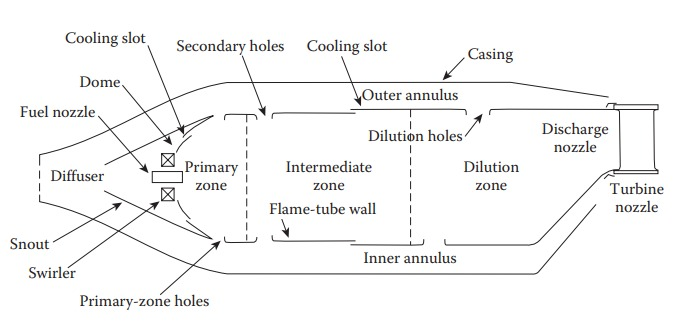
\includegraphics[width=0.8\textwidth]{Chapter1/Images/Conventional combustor.jpeg}
	\caption[Conventional gas turbine combustor.]{Conventional gas turbine combustor \cite{LTY2013}}
	\label{fig:gasTurbineEngine}
\end{figure}

In the combustor, diffuser is used to  reduce the pressure drop, a diffuser is typically used to slow the air as it enters the combustion chamber. Swirlers help to stabilise flames by creating a recirculating flow field in the primary zone. To keep gas temperature within safe range for the turbine blades as it moves downstream from the primary zone, air is injected through liner holes. Temperature profile of the exhaust gases entering the turbine vanes can be modified thanks to this air injection \cite{LAH2010}.

The fundamental requirements for most combustors \cite{LAH2010} are outlined as follows:
\begin{itemize}
    \item \textbf{High combustion efficiency}: The combustion chamber should facilitate complete burning of the injected fuel, ensuring that its entire chemical energy is converted into heat.

    \item \textbf{Wide stability limits}: The combustor needs to operate reliably across a broad range of conditions, including varying pressures and air/fuel ratios.

    \item \textbf{Reliable and smooth ignition}: Aircraft engines must be capable of smooth ignition both on the ground, particularly in cold weather, and at high altitudes where air density is significantly reduced after a flameout.

    \item \textbf{Low pressure loss}: Acceptable pressure loss typically falls within the range of 4-8\%.

    \item \textbf{Uniform temperature profile at the outlet (pattern factor)}: Lifespan of turbine blades can be maximized by uniform distribution of temperature at the outlet.

    \item \textbf{Low emissions}: The gas turbine engines should comply with the pollution control regulations set by international authorities, ensuring minimal pollutant emissions.

    \item \textbf{Free from combustion instabilities}: Combustion instabilities should be minimized to prevent damage to the combustor hardware and ensure stable operation.

    \item \textbf{Compact size}: Combustor design must meet the shape and size requirements of gas turbine engines.

    \item \textbf{Fuel flexibility}: Combustor should be capable of accommodating various fuel types, typically kerosene-based for aircraft gas turbines.

    \item \textbf{Ease of maintenance}: Combustor's geometry should allow for convenient maintenance in the event of any reported issues.
\end{itemize}

\section{Gas Turbine Combustor Design Parameter}
\subsection{High Thermal Intensity}
Equation \ref{thermalIntensity} refers to thermal intensity. In land based gas turbine combustor, typically exhibits a thermal intensity of approximately 5-15 MW/m3-atm. 
\begin{equation}{\label{thermalIntensity}}
    Thermal\ intensity\ = \ \frac{Heat\ release\ rate}{Volume \times Pressure}
\end{equation}
Consequently, high thermal intensity results in high thermal load within a small combustor volume. This is crucial for aerospace applications as it enables space and weight savings in the engine design.

\subsection{Low Pollutant Emission}
Primary pollutants released from the gas turbine combustor include NOx, CO, UHC, and soot. NOx emissions tend to be higher at higher equivalence ratios, reaching a peak at stoichiometric conditions, and decrease in fuel-rich conditions. Conversely, high levels of CO and UHC emissions are observed at both high and low equivalence ratios \cite{AGARWAL20171}. Therefore, there exists a limited range where both NOx and CO emissions remain low and within acceptable limits, as depicted in Figure \ref{PollEq}. Soot, composed of unburnt carbon particles, is primarily generated under fuel-rich conditions.
\begin{figure}[ht]
	\centering
	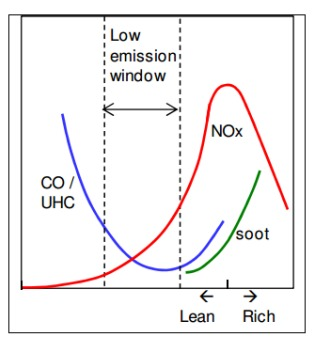
\includegraphics[width=0.5\textwidth]{Chapter1/Images/emissionWithEq.jpeg}
	\caption[Pollutant emissions variation with equivalence ratio]{Pollutant emissions variation with equivalence ratio \cite{SKG2017}.}
	\label{PollEq}
\end{figure}

Level of pollution released by a combustor can be quantified using Emission Index. Emission Index is defined in various ways, such as in grams per kilogram (g/kg) or parts per million by volume (ppm) at a specified O$_2$ concentration. 
\begin{equation}
    Emission\ index_i\ = \frac{Mass\ flow\ rate\ of\ emitted\ species\ (g)}{Mass\ flow\ rate\ of\ fuel\ (kg) }
\end{equation}

This index represents the amount of pollutant generated per unit mass of fuel. In the case of hydrocarbon fuels, Emission Index is determined based on the mole fraction of species containing carbon.
\begin{equation}
    Emission\ index_i\ = \frac{X_i}{X_{CO} + X_{CO_2} + x*X_{UHC}} \frac{(x+2)MW_i}{MW_f}
\end{equation}
Where
\begin{equation*}
    X^s \ = \ \frac{X_i}{X_{CO} + X_{CO_2} + x*X_{UHC}}
\end{equation*} are mole fractions, $MW_i$ and $MW_f$ are the molecular weights of the species i and the fuel \cite{doi:10.2514/6.2012-522}, respectively and $x$ is the number of moles of carbon in a mole of fuel, \cite{doi:10.2514/6.2013-3677}.

\subsection{Pressure Drop}
The major cause of pressure losses within a combustion chamber is primarily attributed to the increase in temperature resulting from the combustion process. Additionally, pressure losses can occur due to cold losses caused by friction and inherent pressure losses. It is essential to minimize pressure drop since it directly affects the loss of thrust generated by the engine. 

\begin{equation}
    Pressure\ drop\ = \ \frac{P_{inlet}- P_{exit}}{P_{inlet}}
\end{equation}

Total pressure at the inlet and exit of the combustor is represented by P$_{inlet}$ and P$_{exit}$, respectively. Typically, the total pressure drop ranges from approximately 4$\%$ to 7$\%$ of the inlet total pressure for aircraft engines, while for land-based gas-turbine combustors, it is around 1$\%$ to 2$\%$ \cite{GTT1996}.

\subsection{Pattern Factor}
Pattern factor, also known as Temperature Traverse Quality, quantifies the non-uniformity of temperature at the turbine inlet (or combustor exit) and is normalized based on the average temprature difference between the exit and inlet. When designing the gas turbine combustion chamber, it is crucial to achieve a suitable and consistent temperature distribution at the turbine exit. The pattern factor directly impacts the engine's power output and the longevity and robustness of the turbine blades located downstream of the combustor.
\begin{equation}
    Pattern\ factor\ = \ \frac{T^{max}_4 - T^{avg}_4}{T^{avg}_4 - T_3}
\end{equation}

In the equation, $T^{max}_4$ denotes the highest temperature achieved at the combustor exit, $T^{avg}_4$ represents the average temperature across the combustor exit, and $T_3$ corresponds to the temperature at the combustor inlet. A pattern factor that approaches zero indicates an ideal scenario with highly uniform temperatures across the combustor exit. Conversely, a pattern factor exceeding 0.4 suggests a non-uniform temperature distribution, which is considered undesirable \cite{mattingly2005elements}.

\subsection{Combustion Efficiency}
The combustion efficiency is a metric that indicates the effectiveness of utilizing the fuel in the combustion process. Coembustion efficiency is defined as \cite{GTT1996}:
\begin{equation}
    Combustoin\ efficiency\ = \ \frac{100}{\Delta H_{CV}}[\Delta H_{CV} - ((\Delta H_{CV} \times EI_{CO}) + (EI_{UHC}\times\Delta H_{CV}))]
\end{equation}
Where $EI_{CO}$ is the emission index of carbon monoxide, $EI_{UHC}$ is the emission index of unburned hydrocarbons, $\Delta H_{CV}$ is the lower heating value of the fuel.

\subsection{Combustion Instability}
Combustion instabilities arise from significant pressure oscillations caused by the interaction between natural acoustic mode and the oscillatory heat release process of the combustor. These oscillations can escalate from small disturbances to sustained limit cycle oscillations. Combustion instabilities become more pronounced close to the lean operational limit of modern ultra-lean premixed or partially premixed combustors. It is crucial to mitigate these instabilities during combustion to prevent fatigue, thermal stress on combustor components, and potential complete failure of the combustor over time.

\subsection{Operational Limit}
The operational limits of a combustion chamber are determined by the minimum and maximum equivalence ratio required to sustain a flame. The lean operational limit refers to the minimum equivalence ratio at which the flame remains stable without blowing off. Conversely, the rich operational limit represents the maximum equivalence ratio at which the flame can be sustained before extinguishing. The actual equivalence ratio within the combustion chamber varies due to mixing effects. A larger difference between lean and rich operational limits indicates greater combustion stability, highlighting the importance of achieving a wider range for enhanced stability in the combustion process.

\section{Pollutant Formation}
One of the most crucial factors to consider is the emission of pollutants from the combustor. It is essential to minimize these emissions due to the stricter aircraft emission standards worldwide. Primary pollutants released from the gas turbine combustor include NOx, CO, UHC, and soot. NOx emissions tend to be higher near stoichiometric stoichiometric conditions, and decrease in fuel-rich conditions. Conversely, at both low and high equivalence ratios, higher CO and UHC emissions are measured. Consequently, there is only a limited range where both CO and NOx emissions are low and within acceptable limits, as illustrated in Figure \ref{PollEq}. Soot comprises unburnt carbon particles and is primarily generated under fuel-rich conditions.

\subsection{Oxides of Nitrogen (NOx)}
Majority of nitric oxide (NO) generated during combustion undergoes oxidation to form nitrogen dioxide (NO$_2$). Due to this, it is common practice to combine NO and NO$_2$ and refer to them collectively as NOx, instead of solely focusing on NO. NOx can be formed in four different mechanism: thermal NOx, prompt NOx, nitrous oxide mechanism, and fuel NOx\cite{Carvalho2024}.


\begin{figure}[h]
	\centering
	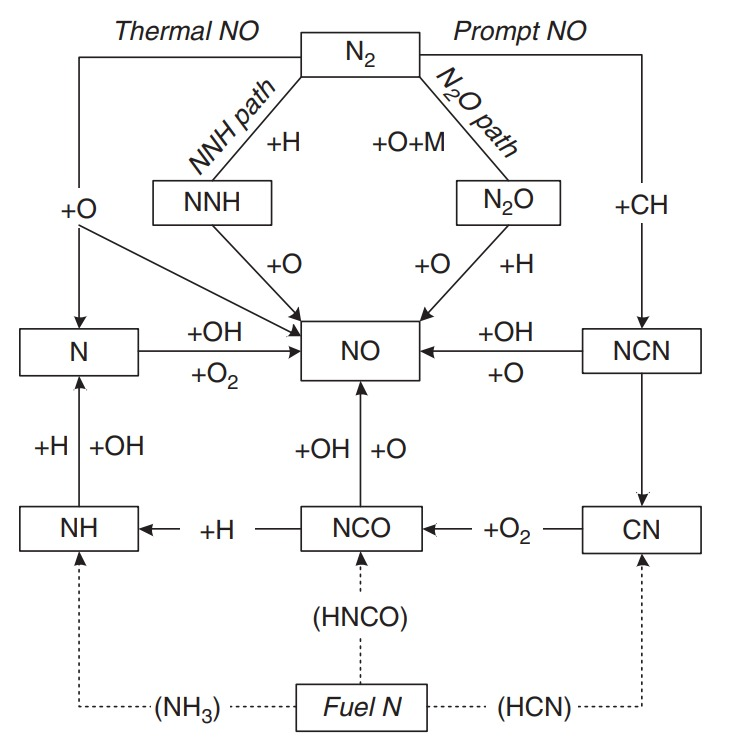
\includegraphics[width=0.6\textwidth]{Chapter1/Images/NoxMechanism.jpeg}
	\caption[Comprehensive NOx formation mechanism]{Comprehensive NOx formation mechanism \cite{LTY2013}.}
	\label{NoxMechanism}
\end{figure}

\subsubsection{Thermal NOx Formation (Zeldovich Mechanism)}
Thermal NOx formation is a prominent mechanism by which nitrogen oxides (NOx) are generated during combustion processes. Understanding this intricate mechanism is vital for developing effective strategies to mitigate NOx emissions and reduce their environmental impact. The following steps help to understand the complex process of thermal NOx formation mechanism:

\textbf{Nitrogen Fixation:}
The thermal NOx formation mechanism begins with the thermal dissociation of atmospheric nitrogen (N$_2$) into individual nitrogen atoms (N*). This dissociation occurs when high temperatures, typically in excess of 1850 K, are reached during combustion. The energy from the combustion process breaks the strong bonds holding the N$_2$ molecules together, resulting in the release of highly reactive nitrogen atoms.

\textbf{Nitric Oxide Formation:}
Once the nitrogen atoms (N*) are generated, they react with oxygen molecules (O$_2$) to form nitric oxide (NO) through a series of intermediate reactions. 

The key steps involved in the development of nitric oxide include:
\begin{itemize}
    \item N$_2$ + O$_2$ → 2NO: The formation of nitric oxide (NO) is mainly driven by the high temperatures reached during combustion. Nitrogen (N$_2$) from the air reacts with oxygen (O$_2$) to produce nitric oxide. This reaction is highly exothermic and occurs rapidly.
    \item N + O$_2$ → NO + O: The nitrogen atom (N) reacts with another oxygen molecule (O$_2$) to produce additional an oxygen atom (O) and nitric oxide (NO). This reaction contributes to the overall formation of nitric oxide.
\end{itemize}

\textbf{Nitrogen Dioxide Formation:}
Once nitric oxide (NO) is formed, it can further react with oxygen to produce nitrogen dioxide (NO$_2$), which is a significant component of NOx emissions.

Formation of nitrogen dioxide involves the following steps:
\begin{itemize}
    \item 2NO + O$_2$ $\longleftrightarrow$ 2NO$_2$: Nitric oxide (NO) reacts with an oxygen molecule (O$_2$) to generate nitrogen dioxide (NO$_2$). 
This reaction is relatively slow compared to the development of nitric oxide.
\item NO$_2$ $\longleftrightarrow$ NO + O: Nitrogen dioxide (NO$_2$) can also dissociate back into nitric oxide (NO) and an oxygen atom (O) through a reversible reaction. 
This equilibrium reaction plays a important role in the combustion system to determining the overall concentration of NO$_2$.
\end{itemize}

\begin{figure}[h]
	\centering
	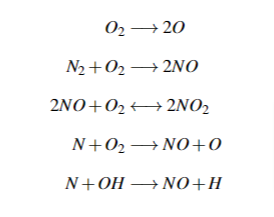
\includegraphics[width=0.4\textwidth]{Chapter1/Images/reaction4.png}
\end{figure}
% \begin{equation*}
%     \begin{split}
%         O_2 &\longrightarrow 2O\\
%         N_2 + O_2 &\longrightarrow  2NO \\
%         2NO + O_2 &\longleftrightarrow 2NO_2 \\
%         N + O_2 &\longrightarrow  NO + O \\
%         N + OH &\longrightarrow  NO + H \\
%     \end{split}
% \end{equation*}

\begin{figure}[h]
	\centering
	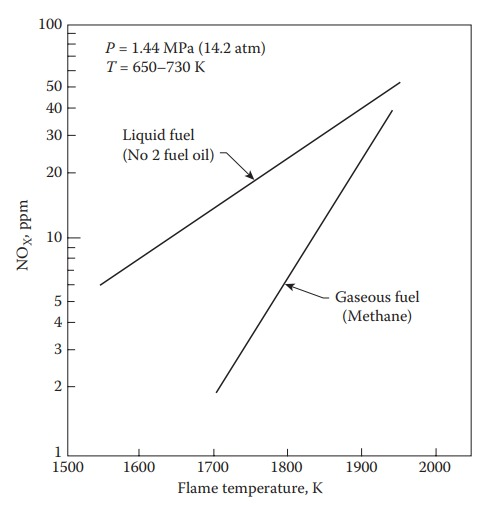
\includegraphics[width=0.7\textwidth]{Chapter1/Images/NoxVsTemp.jpeg}
	\caption[NOx variation with flame temperature for liquid and gaseous fuels]{NOx variation with flame temperature for liquid and gaseous fuels \cite{94-GT-283}.}
	\label{NoxVsTemp}
\end{figure}

\textbf{Impact of Operating Conditions on Thermal NOx Formation:}
Several factors influence the extent of thermal NOx formation during combustion processes. Key factors include:
\begin{itemize}
    \item Temperature: Thermal NOx formation rate increases exponentially with temperature. A high combustion temperature leads to a higher concentration of nitrogen atoms (N*) and, consequently, increased NOx formation, see Figure \ref{NoxVsTemp}.
    \item Oxygen Concentration: Availability of oxygen affects the reactions involving nitrogen atoms and nitric oxide. Insufficient oxygen can lead to the accumulation of nitrogen atoms and a subsequent increase in NOx formation.
    \item Residence Time: The duration that reactant molecules spend within the high-temperature combustion zone, known as the residence time, impacts the overall NOx formation. Longer residence times allow for more extensive nitrogen-oxygen reactions, leading to increased NOx emissions.
    \item Fuel Composition: Nitrogen-containing compounds in fuels (coal or certain liquid fuels) contribute to the overall NOx formation during combustion.
\end{itemize}

\subsubsection{Nitrous Oxide Mechanism}
The following step is initiate the reaction

\begin{figure}[h]
	\centering
	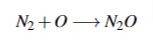
\includegraphics[width=0.2\textwidth]{Chapter1/Images/reaction3.png}
\end{figure}
% \begin{equation*}
% \begin{split}
%     N_2 + O &\longrightarrow N_2 O
% \end{split}
% \end{equation*}
and formed nitrous oxide ($N_2 O$) is then oxidized to NO by the following reaction \cite{Lefebvre2009}.
\begin{figure}[h]
	\centering
	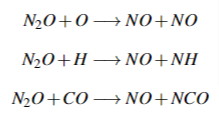
\includegraphics[width=0.3\textwidth]{Chapter1/Images/reaction2.png}
\end{figure}
% \begin{equation*}
%     \begin{split}
%         N_2 O + O &\longrightarrow NO + NO \\
%         N_2 O + H &\longrightarrow NO + NH \\
%         N_2 O + CO &\longrightarrow NO + NCO
%     \end{split}
% \end{equation*}

\subsubsection{Prompt NOx Formation}
Prompt NOx production contributes significantly to NOx emissions in combustion processes, particularly in fuel-rich situations.
The following process highlight the prompt NOx mechanism:

\textbf{Fuel-Rich Combustion Conditions:}
Prompt NOx formation occurs primarily in fuel-rich environments, such as those encountered in certain types of combustion systems like engines and gas turbines. 
In these conditions, availability of fuel is relatively high compared to the available oxygen for combustion, leading to incomplete oxidation of the fuel.

\textbf{Nitrogen Radical Generation:}
During fuel-rich combustion, high temperatures break down nitrogen-containing species in the fuel, such as nitrogen compounds or fuel-bound nitrogen, releasing nitrogen radicals (N*) into the combustion zone. 

Key steps involved in nitrogen radical generation include:
\begin{itemize}
    \item Fuel Decomposition: High temperatures cause the fuel molecules to decompose, releasing reactive hydrocarbon radicals and nitrogen-containing radicals.
    \item Thermal Dissociation: Nitrogen-containing species undergo thermal dissociation, leading to the formation of highly reactive nitrogen radicals (N*).
\end{itemize}

\textbf{Hydrocarbon Radical Reactions:}
In fuel-rich conditions, hydrocarbon radicals present in the combustion zone can react with nitrogen radicals to form prompt NOx species. These reactions contribute to the overall prompt NOx formation. The key pathways of hydrocarbon radical reactions include:
\begin{itemize}
    \item Hydrocarbon-Nitrogen Radical Reaction: Hydrocarbon radicals react with nitrogen radicals (N*) to form prompt NOx species, such as nitroalkanes and alkyl nitrates. Exact reactions involved depend on the specific hydrocarbon radicals and nitrogen radicals present.
\end{itemize}

\begin{figure}[h]
	\centering
	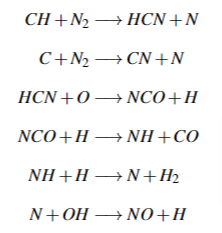
\includegraphics[width=0.3\textwidth]{Chapter1/Images/reaction1.png}
\end{figure}

% \begin{equation*}
%     \begin{split}
%         CH + N_2 &\longrightarrow HCN + N\\
%         C+ N_2 &\longrightarrow CN + N\\
%         HCN + O &\longrightarrow NCO + H\\
%         NCO + H &\longrightarrow NH + CO\\
%         NH + H &\longrightarrow N + H_2\\
%         N + OH &\longrightarrow NO + H\\
%     \end{split}
% \end{equation*}

The extent of prompt NOx formation is influenced by various operating conditions and factors:
\begin{itemize}
    \item Fuel-Richness: The degree of fuel-richness in the combustion environment significantly affects prompt NOx formation. Higher fuel-to-air ratios result in more significant prompt NOx emissions.
    \item Residence Time: The residence time, or the duration that the reactant molecules spend within the fuel-rich zone, impacts the overall prompt NOx formation. Longer residence times allow for more extensive hydrocarbon-nitrogen radical reactions, leading to increased prompt NOx emissions.
    \item Temperature: Although prompt NOx formation is more prominent in fuel-rich conditions, high temperatures still play a role. Increased temperatures enhance the decomposition of nitrogen-containing species and facilitate the generation of nitrogen radicals for reactions with hydrocarbon radicals.
\end{itemize}

\subsubsection{Fuel NOx Formation}
Fuel-bound nitrogen oxides (fuel NOx) play a significant role in the formation of NOx emissions during combustion processes. The following process highlight the fuel NOx mechanism:

\textbf{Nitrogen Compounds in Fuel:}
Many fuels, including coal, oil, and biomass, contain varying amounts of nitrogen compounds. These compounds can be categorized into two main groups: organic nitrogen compounds and inorganic nitrogen compounds. Organic nitrogen compounds are derived from biomaterials and fossil fuels, while inorganic nitrogen compounds include ammonia and nitrates.

\textbf{Nitrogen Release during Combustion:}
When fuel is subjected to high temperatures during combustion, the nitrogen compounds present undergo thermal decomposition, releasing nitrogen species into the combustion zone. The nitrogen species then participate in various reactions, leading to the formation of fuel NOx. 

The key pathways of fuel NOx formation include:
\begin{itemize}
    \item \textbf{Nitrogen Oxide Formation:} Organic nitrogen compounds decompose, releasing nitrogen radicals (N*) into the combustion zone. These nitrogen radicals rapidly react with oxygen molecules (O$_2$) to form nitric oxide (NO). The released nitrogen oxide can further react to form nitrogen dioxide (NO$_2$), which contributes to the overall fuel NOx emissions.
    \item \textbf{Nitrogen-Atom Transfer:} Inorganic nitrogen compounds, such as ammonia (NH$_3$), decompose into nitrogen atoms (N*). These nitrogen atoms reaction with oxygen or other reactive species in combustion chamber, can lead to form nitric oxide (NO). This process is known as nitrogen-atom transfer and is a significant contributor to fuel NOx emissions.
    \item \textbf{Nitrous Oxide Formation:} Some fuel nitrogen compounds, particularly nitrogen-based heterocyclic compounds found in coal and biomass, can also contribute to the formation of nitrous oxide (N$_2$O) during combustion. Nitrous oxide is a potent greenhouse gas and a minor contributor to fuel NOx emissions.
\end{itemize}

The fuel NOx formation is influenced by several fuel-related factors:
\begin{itemize}
    \item Fuel Nitrogen Content: The nitrogen content of the fuel plays a crucial role in determining the potential for fuel NOx formation. Fuels with higher nitrogen content have a higher propensity to generate fuel NOx emissions.
    \item Fuel Composition: Different fuel types contain varying organic and inorganic nitrogen compounds, leading to differences in the fuel NOx formation potential. For example, coal generally contains higher nitrogen content compared to natural gas, resulting in higher fuel NOx emissions when combusted.
    \item Fuel Processing: Fuel processing techniques, such as desulfurization and denitrification, can reduce the amount of nitrogen in the fuel and subsequently lower the fuel NOx formation potential.
\end{itemize}

\subsection{CO (UHC) formation}
It typically emerges when the combustion zone operates in a fuel-rich state, where there isn't enough oxygen for complete conversion to CO$_2$. CO is produced significantly even under stoichiometric conditions or slightly fuel-lean conditions due to the dissociation of CO$_2$. In lean conditions, characterized by a slow burning rate, CO levels tend to be high because of the slower conversion of CO to CO$_2$, where the time spent in the combustion process is a crucial factor. It has been observed that there is a correlation between CO and UHC emissions, as the factors influencing CO also affect UHC \cite{LAH2010}.

\subsection{Soot Formation}
Soot formation occurs through a complex series of chemical reactions during the combustion process. The key steps involved in the formation of soot particles are:
\begin{itemize}
    \item \textbf{Fuel Pyrolysis:} When fuel is exposed to high temperatures in the presence of limited oxygen, it undergoes pyrolysis, breaking down into smaller hydrocarbon fragments.
    \item \textbf{Nucleation:} In regions of fuel-rich environments, small carbonaceous particles begin to form through nucleation. These particles are primarily composed of polycyclic aromatic hydrocarbons (PAHs) and other carbon-rich species.
    \item \textbf{Surface Growth:} The nucleated particles grow by absorbing other hydrocarbons present in the combustion environment. The growth occurs through the deposition of additional carbon onto the existing particles, resulting in larger and more complex structures.
    \item \textbf{Aggregation:} The grown soot particles may aggregate with each other, forming larger agglomerates.
    \item \textbf{Soot Oxidation:} In the presence of oxygen, soot particles can undergo oxidation, which can result in the eventual destruction of the particles. However, in fuel-rich environments with limited oxygen availability, this oxidation process is inhibited, leading to the accumulation of soot.
\end{itemize}

Several factors affect the formation of soot in combustors, including:
\begin{itemize}
    \item \textbf{Fuel Composition:} The chemical composition of the fuel significantly influences soot formation. Fuels with higher carbon content, such as heavy oils or coal, are more prone to soot formation compared to cleaner fuels like natural gas or hydrogen.
    \item \textbf{Air-Fuel Ratio:} The air-fuel ratio plays a crucial role in soot formation. Fuel-rich conditions, where there is an insufficient supply of oxygen for complete combustion, promote soot formation. Insufficient oxygen limits the availability of oxidants needed for complete combustion and encourages the formation of carbonaceous particles.
    \item \textbf{Residence Time:} The residence time, or the duration that fuel spends in the combustor, also impacts soot formation. Longer residence times provide more opportunities for incomplete combustion and subsequent soot formation.
    \item \textbf{Temperature:} The temperature profile within the combustor affects soot formation. High temperatures can enhance the pyrolysis process, leading to increased soot precursor formation. Additionally, inadequate mixing of fuel and air can result in localized regions of lower temperatures that favor soot formation.
\end{itemize}

\section{Nomenclature for different flow configurations}
Figure \ref{FlowConfig} shows different flow configurations of CDC combustor, where A represents air port, B represents exit port and F indicate fuel port. In chapter \ref{CH2:LTR}, different flow configuration are discussed for various combustion technologies. In the present study also, we will discuss reverse flow configuration for premixed and non-premixed cases.
\begin{figure}[ht]
	\centering
	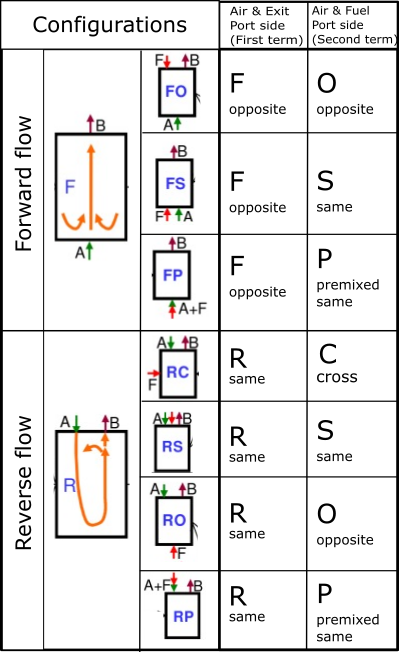
\includegraphics[width=0.7\textwidth]{Chapter1/Images/FlowConfiguration.png}
	\caption[Flow configurations of CDC combustor]{Flow configurations of CDC combustor \cite{VAThesis2011}.}
	\label{FlowConfig}
\end{figure}